\documentclass[grad,pdftex]{poli}
\usepackage[utf8]{inputenc}
\usepackage{amsmath,amssymb}
\usepackage{indentfirst}
\usepackage{graphicx}
\usepackage{appendix}
%\usepackage[colorinlistoftodos]{todonotes}
\usepackage{listings}
\usepackage{color}
\usepackage{subcaption}
\usepackage{float}
\usepackage{animate}
\usepackage{hyperref}

\definecolor{dkgreen}{rgb}{0,0.6,0}
\definecolor{gray}{rgb}{0.5,0.5,0.5}
\definecolor{mauve}{rgb}{0.58,0,0.82}

\lstset{frame=tb,
  language=Python,
  aboveskip=3mm,
  belowskip=3mm,
  showstringspaces=false,
  columns=flexible,
  basicstyle={\small\ttfamily},
  numbers=none,
  numberstyle=\tiny\color{gray},
  keywordstyle=\color{blue},
  commentstyle=\color{dkgreen},
  stringstyle=\color{mauve},
  breaklines=true,
  breakatwhitespace=true,
  tabsize=3
}

\makelosymbols
\makeloabbreviations

\begin{document}
  \title{Titulo da Tese}
  \foreigntitle{Solution of Generalized Eigensystems with Algorithms Based on
  Arnoldi Methods}
  \author{Estudante}{Dedicado}
  \advisor{Prof.}{Professor}{Dorminhoco}{D.Sc.}
  \coadvisor{Prof.}{Professor}{Atarefado}{Dr.-Ing.}
  \examiner{Prof.}{}{D.Sc.}
  \examiner{Prof.}{}{Ph.D.}
  \examiner{Prof.}{}{D.Sc.}
  \department{DEM}
  \date{10}{2021}
  \keyword{Redes Neurais}
  \keyword{Mecânica dos Fluidos}
  \keyword{Darcy}
  \maketitle

  \frontmatter
  \dedication{Aos amigos dedicados da Mecânica\\
 (\emph{Vcs conseguem}).}


  \chapter*{Agradecimentos}

Blablabla sem fim. Agradece a mãe o pai piriquito e papagaio


  \begin{abstract}

Este trabalho apresenta o desenvolvimento de um simulador \textit{web} interativo para análise cinemática de um manipulador robótico de seis graus de liberdade (6-DOF), voltado ao apoio didático em disciplinas de automação e robótica. A ferramenta, executada diretamente no navegador, implementa modelagem baseada na Convenção de \textit{Denavit–Hartenberg}, permitindo a realização de cinemática direta e inversa, além de planejamento de trajetória por interpolação polinomial cúbica. O sistema possibilita o controle individual das juntas ou do posicionamento cartesiano do efetuador final, bem como a visualização em tempo real da matriz de transformação homogênea e dos gráficos de posição, velocidade e aceleração angular. Não serão abordados aspectos relativos à dinâmica de manipuladores.

Palavras-chave: Simulação, robótica, trajetória, cinemática.

\end{abstract}


  \begin{foreignabstract}

Aqui você resume o seu projeto, só que \textit{in english}

\end{foreignabstract}


  \tableofcontents
  \listoffigures
  \listoftables
  \printlosymbols
  \printloabbreviations

  \mainmatter
  \chapter{Introdução}

Lorem ipsum dolor sit amet, consectetur adipiscing elit. Vivamus in imperdiet urna. Quisque convallis vel neque quis finibus. Duis finibus velit nulla, id tincidunt lacus mattis sit amet. Nulla facilisi. Sed sit amet nibh tristique nisl volutpat fermentum. Sed porta pulvinar ligula, sit amet maximus nibh gravida id. Nulla ac justo hendrerit, hendrerit nibh sed, blandit augue.

Donec eu aliquet metus, eu malesuada ligula. Ut efficitur ut ligula at sollicitudin. Proin sed mauris eget ligula ultricies consectetur in nec risus. Aliquam non sapien at nisi mollis fringilla ut et mauris. Cras volutpat justo in leo congue, non gravida velit volutpat. Donec laoreet pellentesque mi, ac rhoncus mi dignissim vel. Sed quis nibh velit.

Nullam at dignissim lacus. Donec euismod malesuada vehicula. Sed molestie est a nisi sollicitudin tempor. Fusce tincidunt libero sed felis lacinia volutpat. Nulla eu auctor turpis. Curabitur et nisl id ante laoreet facilisis. Aenean egestas, arcu non viverra auctor, magna mauris consequat ligula, vitae rutrum nulla lacus in dui. Integer accumsan libero nulla, vel varius magna finibus et. Aliquam erat volutpat. In et ligula id nibh faucibus bibendum. Curabitur ornare lectus eu orci placerat, vitae pretium enim ultricies. Nulla quis enim eget est venenatis imperdiet. Maecenas mattis urna porttitor, pretium orci eu, vulputate nunc. Mauris vestibulum interdum dictum. Cras scelerisque congue lorem a rhoncus.

Pellentesque id ex egestas, feugiat nunc ut, pellentesque justo. Maecenas ligula mi, sagittis eu aliquet at, gravida nec libero. Fusce pulvinar, tortor vel scelerisque porttitor, erat urna sollicitudin purus, tempor sagittis mauris libero a quam. Proin nec nisi suscipit, sodales enim ultricies, mattis metus. Mauris sed tellus tellus. Suspendisse pellentesque metus vitae nulla mollis imperdiet. In hac habitasse platea dictumst. Sed lorem quam, ultricies vel nulla vitae, porttitor consequat nunc. Etiam eu lectus nunc.

Curabitur rutrum lobortis vehicula. Duis eros nisl, blandit non nisi et, efficitur ultricies tortor. Nullam faucibus quam dolor, at auctor dui consectetur sed. Suspendisse dapibus nec arcu in mollis. In fermentum hendrerit leo id commodo. Mauris fringilla mollis velit aliquet lobortis. Mauris quis ligula a arcu vehicula convallis et sed magna. Nunc ac placerat eros, id fringilla nisl. Sed consectetur aliquam malesuada. Aenean rutrum enim nec tortor ultrices, id fermentum nunc varius. Duis rhoncus eu dolor in ullamcorper. Nulla enim mauris, facilisis quis nunc at, egestas tempus risus. Aenean rutrum fringilla ultricies. Phasellus vel euismod dui. Donec egestas bibendum interdum.


\section{Motivaç{\~ a}o}

Aqui vc fala seus motivos, por mais loucos que eles sejam, para você ter escolhido esse assunto tão interessante que eu sei que é o tema do seu Projeto.

\section{Objetivo}

Uma vez eu construí um motor Stirling de latinha de coca cola e queria fazer um fogão solar pra acioná-lo. O objetivo no caso era construir um motor que não utilizasse produtos químicos como combustível.

\section{Metodologia}

Pra fazer esse motor eu usei duas latinhas, cortei a primeira numa altura de 6cm e retirei a tampa, usei um raio de bicicleta para construir o virabrequim, o pistão foi feito com um pedaço do raio, lã de aço e as tampas retiradas das latinhas...

\section{Organizaç{\~ a}o da tese}

Preferi organizar assim assim e assado, este é um exemplo de equação:

\begin{equation}\label{equacao}
    x = \theta y
\end{equation}

Para criar um símbolo na sua lista de símbolos, basta utilizar o comando symbl com dois parâmetros, sendo o primeiro o símbolo, utilizando \$ para denotar o modo matemática no LaTeX. e o segundo parâmetro sendo a descrição do símbolo.

\symbl{$\theta$}{coeficiente angular}

Deste outro jeito, escrevo a equação sem numerá-la:

\begin{equation*}
    x = y
\end{equation*}

Se eu quiser referenciar minha equação, basta utilizar este comando: \ref{equacao}

Este é um template da COPPE, que é uma abreviação para Instituto Alberto Luiz Coimbra de Pós-Graduação e Pesquisa de Engenharia. Para criar abreviações na sua lista de abreviações, basta utilizar o commando abbrev, com dois parâmetros, sendo o primeiro a abreviação e o segundo a descrição.

\abbrev{COPPE}{Instituto Alberto Luiz Coimbra de Pós-Graduação e Pesquisa de Engenharia}
  \chapter{Revisão Bibliográfica}

Aqui eu falo um monte das referências bibliográficas, pra cada coisa que eu falar aqui, eu vou ter que citar alguém. Dessa maneira: \cite{Lan50a}

  \chapter{Fundamentação Teórica}

\section{Métodos Utilizados}
\subsection{Método de Newton}

Pode ser necessário utilizar uma figura para explicar alguma coisa, tal como mostrar algum método, como o método de Newton para aproximação de uma função, que consiste em realizar esta aproximação através da função tangente, como mostra a figura

\begin{figure}[H]
    \centering
    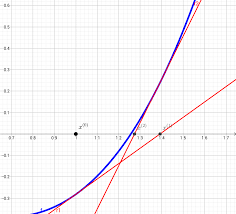
\includegraphics{Imagens/newton-method.png}
    \caption{Exemplo de utilização do método de Newton}
    \label{fig:newton}
\end{figure}

A tag [H] serve para posicionar a figura na posição exata do texto, caso contrário, a mesma poderá aparecer como objeto flutuante em regiões indesejadas devido a erros no LaTEX.
Para referenciar a figura, basta utilizar o comando ref, desta forma: \ref{fig:newton}



  \include{Textual/chap04}
  \include{Textual/chap05}

  \backmatter
  \nocite{*}
  \bibliographystyle{poli-unsrt}
  \bibliography{thesis}
  \appendix
  \chapter{Código Fonte}

\begin{lstlisting}
def hello_world():
    print("Hello world!")
    ## Este eh um exemplo de codigo comentado
    return true
\end{lstlisting}
\end{document}
